%-----------------------------------------------------------------------------
%
%               Template for sigplanconf LaTeX Class
%
% Name:         sigplanconf-template.tex
%
% Purpose:      A template for sigplanconf.cls, which is a LaTeX 2e class
%               file for SIGPLAN conference proceedings.
%
% Guide:        Refer to "Author's Guide to the ACM SIGPLAN Class,"
%               sigplanconf-guide.pdf
%
% Author:       Paul C. Anagnostopoulos
%               Windfall Software
%               978 371-2316
%               paul@windfall.com
%
% Created:      15 February 2005
%
%-----------------------------------------------------------------------------

\documentclass{sigplanconf}

% The following \documentclass options may be useful:

% preprint      Remove this option only once the paper is in final form.
%10pt          To set in 10-point type instead of 9-point.
% 11pt          To set in 11-point type instead of 9-point.
% authoryear    To obtain author/year citation style instead of numeric.

\usepackage{amsmath}
\usepackage{epsfig}
\usepackage{alltt}
\usepackage{times}
\usepackage{array}
\usepackage{algorithm}
\usepackage{algorithmic}
\usepackage{graphicx}

\newlength\myindent
\setlength\myindent{1em}
\newcommand\bindent{
  \begingroup
  \setlength{\itemindent}{\myindent}
  \addtolength{\algorithmicindent}{\myindent}
}
\newcommand\eindent{\endgroup}

\newlength\mysecindent
\setlength\mysecindent{2em}
\newcommand\quadindent{
  \begingroup
  \setlength{\itemindent}{\mysecindent}
  \addtolength{\algorithmicindent}{\mysecindent}
}
\newcommand\quadeindent{\endgroup}


\begin{document}

\special{papersize=8.5in,11in}
\setlength{\pdfpageheight}{\paperheight}
\setlength{\pdfpagewidth}{\paperwidth}


\doi{}

% Uncomment one of the following two, if you are not going for the 
% traditional copyright transfer agreement.

%\exclusivelicense                % ACM gets exclusive license to publish, 
                                  % you retain copyright

%\permissiontopublish             % ACM gets nonexclusive license to publish
                                  % (paid open-access papers, 
                                  % short abstracts)

\titlebanner{banner above paper title}        % These are ignored unless
\preprintfooter{short description of paper}   % 'preprint' option specified.

\title{Parallel Implementation of Approximate Solvers for Regression using Galois and OpenMP}

\authorinfo{Abhishek Agarwal}
           {University of Texas at Austin}
           {abhishek.agarwal@utexas.edu}
\authorinfo{Ankit Goyal}
           {University of Texas at Austin}
           {ankit3goyal@gmail.com}
\authorinfo{Prateek Agarwal}
           {University of Texas at Austin}
           {prat0318@gmail.com}

\maketitle

\begin{abstract}
The main focus of this work is to solve the problem of Regression for Sparse Data-sets using the Galois framework.
Two different solvers; Gradient and Coordinate descent and their stochastic versions are implemented. The
algorithms are parallelized using OpenMP and Galois framework and their performance and accuracy are compared.
The Tao Analysis for the two solvers is presented and Speedup is compared for different Galois worklist scheduling. A
comparative analysis is presented for change in error loss with respect to the number of iterations and threads. 
\end{abstract}


\keywords
Machine Learning, Stochastic, Gradient, Speedup, Scalability, Ridge Regression, Lasso, Elastic Net, TAO Analysis, Learning Rate, Overfitting, 
Regularization.

\section{Introduction}
Regression, which is a key problem in the field of machine learning, is a statistical process for estimating the relationships among variables. 
Different Models like Least Squares, Ridge Regression and Lasso are used for Regression; of which Least Squares and Ridge Regression have
closed form solutions. An exact solution can be obtained using various Exact solvers which heavily rely on matrix computation libraries. 
Due to complex matrix computations, Exact solvers are unscalable for a large number of features. Thus, approximate solvers like Coordinate Descent 
and Gradient Descent are used when the size of datasets is huge. Since processing all sample values for every feature in an iteration may be computationally
very expensive, Stochastic Methods are used which process either one sample or one feature in an iteration. The Stochastic versions are inherently
sequential in their original form as each iteration is dependent on the values generated by the previous iterations. Thus, slightly modified
versions of Stochastic Gradient and Coordinate Descent have been developed where a random set of samples/features is processed every iteration.\\

The algorithms were parallelized using OpenMP and Galois and the Error loss function values were compared with Scikit Learn. TAO Analysis
of the algorithms is presented and different Galois Worklist Scheduling policies were used to measure performance. Two benchmarks, one sparse and one 
dense were used to compare the runtimes and speedup of the implementations.

\section{Related Work}
With the current advances in multicore processing and the existing need for processing huge web-scale data sets has motivated 
researchers to develop schemes for the parallelization of various machine learning algorithms. Parallelization of the various Regression 
methods continue to be an area of active research. Gradient Descent and Coordinate Descent solvers for regression are embarassingly parallel 
as different samples/features can be processed in parallel during each iteration. The parallelization of their Stochastic versions is more
interesting since only one sample/feature is processed in each iteration. \cite{zhang1} proves the convergence for the standard and averaged 
versions of SGD. However, if locks are implemented to synchronize the threads after each iteration, the scalability of the algorithm is heavily
compromised. Hogwild \cite{hogwild} aims to show using novel theoretical analysis, algorithms, and implementation that SGD can be implemented
without any locking. \\

Several papers have been written studying the iteration complexity of serial and parallel Coordinate Descent Methods(CDMs) in various settings.
Classical CDMs update the weight vectors in a cyclic order whereas in Stochastic/randomized CDMs, the coordinate to be updated is chosen randomly.
\cite{pcd1} shows that randomized (block) coordinate descent methods can be accelerated by parallelization when applied to the problem 
of minimizing the sum of a partially separable smooth convex function and a simple separable convex function. 
\cite{tewari} and \cite{shotgun} apply the Stochastic Methods for \begin{math}l1 \end{math} Regularized Loss Minimization. 
To the best of our knowledge, this is the first attempt at implementing parallel Regression Algorithms using Galois.

\section{Regression}
\noindent
Regression models and analyzes the correlation of several variables. Given a set of training examples 
\begin{math}(x_1,y_1),....,(x_n,y_n)\end{math} where \begin{math} x_i \in R^n \end{math}
and \begin{math} y_i \in (-1,1) \end{math},the goal is to learn a linear scoring function
\begin{math} f(x) = w^Tx + b \end{math} with model parameters \begin{math} w \in R^m \end{math}
and intercept \begin{math} b \in R. \end{math}\\

\noindent
A common choice to find the model parameters is by minimizing the regularized training error given by\\
\begin{equation} E(w,b) = \sum_{i=1}^{n} L(y_i,f(x_i)) + \alpha R(w) \end{equation} \\
where L is a loss function that measures models' (mis)fit and \begin{math}R\end{math} is a
regularization term (aka penalty) that penalizes model complexity; \begin{math}\alpha>0\end{math}
is a non-negative hyperparameter.

\section{Models for Regression}
\subsection{Least Squares}
The best fitting curve to a set of data points could be obtained using least square method. The method
assumes that the best-fit curve for a given data has the minimal sum of the deviations squared. It could
be represented as a minimization problem. For Least squares, the regularization function \begin{math}R(w)=0\end{math}
such that the error is given by \\
\begin{equation} E(w,b) =\frac{1}{2} \sum_{i=1}^{n} (y-Ax)^2\end{equation}
Least Squares has the problem of Overfitting leading to a model that fits the training data very well, but does not generalize well (predict accurately for new examples).

\subsection{Regularization for Regression}
Regularization refers to a process of introducing additional information in order to solve an ill-posed problem or to prevent overfitting. 
This information is usually of the form of a penalty for complexity, such as restrictions for smoothness or bounds on the vector space norm.
For Regression, various Regularization models are used as described next.

\subsubsection{Ridge Regression}
Ridge regression penalizes the size of the regression coefficients. Applying the ridge regression penalty
has the effect of shrinking the estimates (introducing bias but reducing the variance of the estimate). The Error
function is given by \\
\begin{equation} E(w,b) =\frac{1}{2} \sum_{i=1}^{n} (y-Ax)^2 + \sum_{i=1}^{n} w_i^2 \end{equation} \\
The Regularization function is
\begin{equation}R(w)=\frac{1}{2} \sum_{i=1}^{n} w_i^2\end{equation}.

\subsubsection{Lasso}
Ridge regression is capable of reducing the variability and improving the accuracy of linear regression
models, and that these gains are largest in the presence of multicollinearity. However ridge regression
doesn't do variable selection, and it fails to provide a parsimonious model with few parameters.
LASSO is a regression method that penalizes the absolute size of the regression coefficients. It has
desirable effect of setting coefficients to zero leading to sparse solutions.\\
\begin{equation} E(w,b) =\frac{1}{2} \sum_{i=1}^{n} (y-Ax)^2 + \sum_{i=1}^{n} w_i \end{equation} \\
The Regularization function is
\begin{equation}R(w)=\sum_{i=1}^{n} |w_i|\end{equation}.

\subsection{Elastic Net}
Elastic net is a linear model that allows for learning a sparse model where few of the weights are nonzero
like Lasso, while still maintaining the regularization properties of Ridge. The Error function is given by
\begin{equation}E(w,b) =\frac{1}{2} \sum_{i=1}^{n} (y-Ax)^2 + \sum_{i=1}^{n} w_i^2 + \sum_{i=1}^{n} w_i \end{equation} \\
The Regularization function is
\begin{equation}R(w) = \gamma \frac{1}{2} \sum_{i=1}^{n} w_i^2 + (1-\gamma)\sum_{i=1}^{n} |w_i|\end{equation}.

\section{Solvers for Regression}
\subsection{Exact Solvers}
Exact solvers for Regression use various libraries for matrix computation and linear algebra operations.
Default BLAS \cite{blas} and LAPACK, used by Octave and Intel Math Kernel Library (Intel MKL), used by Matlab
are used for obtaining exact solutions for Regression problems. For samples n and d features, the closed form
solution is of the order \begin {math} O(nd^2 + d^3) \end {math} time and \begin {math} O(d^2) \end {math} space for linear regression.
Thus, it is highly unscalable for large number of features d. For the same reason, exact solvers have not been
evaluated in this work and the further analysis would focus on approximate solvers.

\subsection{Gradient Descent}
To find a local minimum of a function using gradient descent, one takes steps proportional to the negative of 
the gradient (or of the approximate gradient) of the function at the current point. The gradient of the error 
function is taken w.r.t one sample at a time and the new weight value for all features is computed.
At the end of the iteration, the final weight values are updated with the mean of weight values calculated using all samples.

\begin{algorithm}
\caption{	Gradient Descent}
\begin{algorithmic} 

\STATE \bf{INPUT} \begin{math} X \in {R}^{N \times  d}, y \in R^N, learning\;  rate\;  \eta, intial\; w \end{math} 
\STATE \bf{OUTPUT} \textnormal{Solution} \begin{math}  w \end{math} 
	\STATE \textnormal{\begin{math} t = 0\end{math} }
	\STATE \bf{while} \textnormal{not converged} \bf{do}
    	\bindent
		 \STATE \bf{for} \textnormal{\indent training example \begin{math}1,2,3..k\end{math}}
		\quadindent
			 \STATE \textnormal{\indent Compute gradient for \begin{math}x_i: \bigtriangledown{E_w(x_i)}\end{math}}
			 \STATE \textnormal{\indent Update \begin{math}w: w^{(t+1)} \gets w^{(t)} - \bigtriangledown{E_w(x_i)}\end{math}}
			 \STATE \textnormal{\indent \begin{math}t \gets t + 1\end{math}}
		\quadeindent
	 \STATE \bf{end for}
	 \eindent
\STATE \bf{end while}

\end{algorithmic}
\end{algorithm}



\subsection{Stochastic Gradient Descent}
In stochastic (or "on-line") gradient descent, the true gradient of the function is approximated by a gradient at a
single training sample. The training samples are given one at a time. The algorithm examines the
current datapoint, and then updates the weight vector accordingly. Thus, it is different from Gradient Descent where the weight
vector is updated with the mean of all samples.





\begin{algorithm}
\caption{Stochastic Gradient Descent}
\begin{algorithmic} 

\STATE \bf{INPUT} \begin{math} X \in {R}^{N \times  d}, y \in R^N, learning\;  rate\;  \eta, intial\; w \end{math} 
\STATE \bf{OUTPUT} \textnormal{Solution} \begin{math}  w \end{math} 

	\STATE \textnormal{\begin{math} t = 0\end{math} }

	\STATE \bf{while} \textnormal{not converged} \bf{do}
    	\bindent
	 \STATE \textnormal{\indent choose a random training example \begin{math}x_i\end{math}}

	 \STATE \textnormal{\indent Compute gradient for \begin{math}x_i: \bigtriangledown{E_w(x_i)}\end{math}}
	 \STATE \textnormal{\indent Update \begin{math}w: w^{(t+1)} \gets w^{(t)} - \bigtriangledown{E_w(x_i)}\end{math}}
	 \STATE \textnormal{\indent \begin{math}t \gets t + 1\end{math}}
	    \eindent
	\STATE \bf{end while}

\end{algorithmic}
\end{algorithm}

\subsection{Coordinate Descent}
As described in \cite{pcd1}, Coordinate descent methods (CDM) are one of the most successful classes of algorithms in the big data optimization domain. 
Broadly speaking, CDMs are based on the strategy of updating a single coordinate (or a single block of coordinates) of the vector
of variables at each iteration. This often drastically reduces memory requirements as well as the
arithmetic complexity of a single iteration, making the methods easily implementable and scalable.
On the other hand, many more iterations are necessary for convergence than it is usual for classical gradient methods.
Coordinate descent is a non-derivative optimization algorithm. To find a local minimum of a function, one does line 
search along one coordinate direction at the current point in each iteration. One uses different coordinate directions 
cyclically throughout the procedure. On non-separable functions the algorithm may fail to find the optimum in a reasonable 
number of function evaluations. 
Coordinate descent is based on the idea that the minimization of a multi-variable function can be
achieved by minimizing it along one direction at a time. Its different from the gradient descent as instead of varying descent direction according
to gradient, one fixes descent direction at the outset.
\begin{algorithm}
\caption{Coordinate descent}
\begin{algorithmic} 
\STATE let $w = 0$
\STATE \bf{for} \begin{math} k = 1,2,.. \end{math}
    \bindent
	\STATE \bf{for} \textnormal{\begin{math}j\end{math} in \begin{math}\{1,...,2d\}\end{math}}
		\quadindent
	\STATE \textnormal{let \begin{math}g_j = (\bigtriangledown{E(w)})_j\end{math}}
	\STATE \textnormal{let \begin{math}\eta = max\{ -w_j, -g_j/\beta \}\end{math}}
	\STATE \textnormal{let \begin{math}w_j = w_j + \eta\end{math}}
	\quadeindent
	\STATE \bf{end for}
    \eindent
\STATE \bf{end for}
\end{algorithmic}
\end{algorithm}

\subsection{Stochastic Coordinate Descent}
If the number of features and data sets is large, going over all dimensions in each iteration is an
expensive approach. In Stochastic Coordinate Descent, only one feature is updated at each iteration. The 
features to be updated can be choosen randomly or in a cyclic manner. The algorithm used for SCD is 
described below.


\begin{figure}[ht!]
\centering
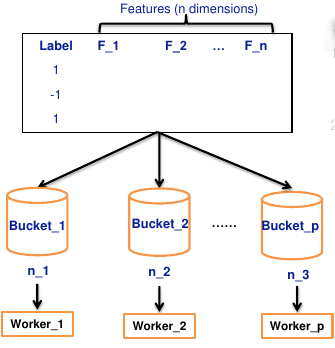
\includegraphics[width=70mm]{openmp_chunked.png}
\caption{Openmp Chunked data access pattern by multiple threads}
\label{overflow}
\end{figure}



\begin{algorithm}
\caption{Stochastic coordinate descent}
\begin{algorithmic} 
\STATE let $w = 0$
\STATE \bf{for} \begin{math} k = 1,2,.. \end{math}
    \bindent
	\STATE \textnormal{sample \begin{math}j\end{math} uniformly at random from \begin{math}\{1,...,2d\}\end{math}}
	\STATE \textnormal{let \begin{math}g_j = (\bigtriangledown{E(w)})_j\end{math}}
	\STATE \textnormal{let \begin{math}\eta = max\{ -w_j, -g_j/\beta \}\end{math}}
	\STATE \textnormal{let \begin{math}w_j = w_j + \eta\end{math}}
    \eindent
\STATE \bf{end for}
\end{algorithmic}
\end{algorithm}

\section{Implementation Framework}
\subsection{OpenMP}
The OpenMP \cite{openmp} is an API that supports multi-platform shared memory multiprocessing programming in C, C++, and Fortran, on most processor architectures and operating systems, including Solaris, AIX, HP-UX, GNU/Linux, Mac OS X, and Windows platforms. It consists of a set of compiler directives, library routines, and environment variables that influence run-time behavior. OpenMP uses a portable, scalable model that gives programmers a simple and flexible interface for developing parallel applications for platforms ranging from the standard desktop computer to the supercomputer. OpenMP 2.5 was used for the parallel
implementation of the algorithms.

\subsection{Galois System}
Galois \cite{galois1}, \cite{galois2} is a system that automatically executes "Galoized" serial C++ or Java code in parallel on shared-memory machines. It works by exploiting amorphous data-parallelism, which is present even in irregular codes that are organized around pointer-based data structures such as graphs and trees. Galois allows the programmer to write serial C++ or Java code while still getting the performance of parallel execution. All the programmer has to do is use Galois-provided data structures, which are necessary for correct concurrent execution, and annotate which loops should be run in parallel. The Galois system then speculatively extracts as much parallelism as it can. The paper analyses the effect of using different Galois schedules for the implementation. 

\subsection{Scikit Learn}
Scikit Learn \cite{scikit} consits of simple and efficient tools for data mining and data analysis implemented in Python. It is open source and commercially usable with a BSD license. For the purpose of this work, scikit was used to compare the Error loss function obtained from sckit with our implementation for the same datasets.

\subsection{RunTime Environment}
The Algorithms were run on the Stampede machine which is one of the largest computing systems in the world for open science research. As an NSF HPC acquisition, this system provides unprecedented computational capabilities to the national research community enabling breakthrough science that has never before been possible. The scale of Stampede delivers opportunities in computational science and technology research, from highly parallel algorithms to high-throughput computing, from scalable visualization to next generation programming languages. It boasts of a total of 6400 nodes with each nodes consisting of 16 cores and a total mememory of 205 TB. Since both OpenMP and Galois are shared memory based, a maximum of 16 cores were used for all runs.

\section{Datasets}
\subsection{Mnist}
\begin{figure}[ht!]
\centering
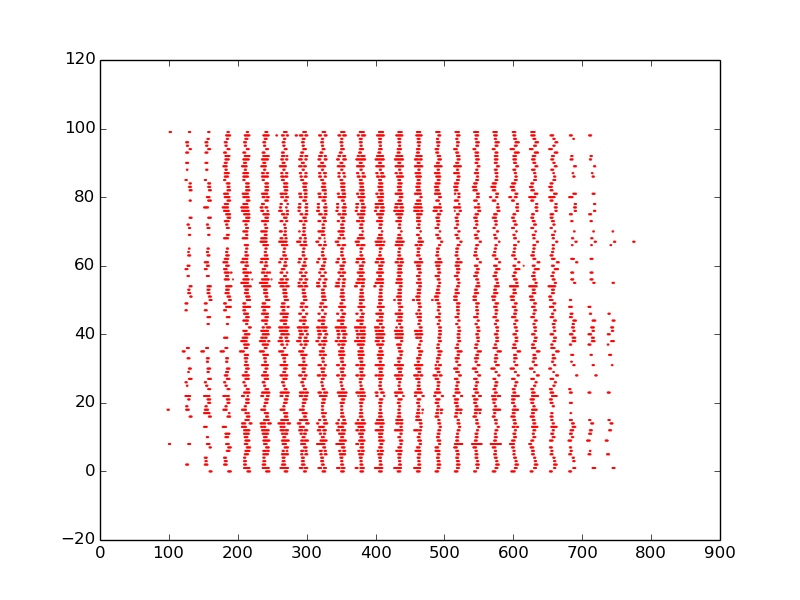
\includegraphics[width=80mm]{mnist_scatter.png}
\caption{Sparse representation of a small set of samples from MNIST. X axis represents the feature present, Y axis represents a sample for which features are present. }
\label{overflow}
\end{figure}

MNIST is a sparse dataset(9\% of the total data-set are non-zero values). This data was primarily built for classification analysis. The database was constructed from NIST's Special Database 3 and Special Database 1 which contain binary images of handwritten digits. The variable set consists of all pixels used to form the digit image. We transformed the data for regression by selecting only two digit samples, namely 1 and 9 and then using it as a binary regression. Samples for 1 were given a Y value of 1 and samples for 9 were given a Y value of -1. Total feature size of the samples is 800 and the total number of samples used were around 0.5 million (513280 samples). Value of any X feature lies in the range(0,255).

\subsection{Madelon}
Madelon is a dense dataset, with number of features kept comparable to the number of samples. It was generated by the program hypercube\_data.m. Some co-variance is added by multiplying the generated data by a random matrix A, with uniformly distributed random numbers between -1 and 1. The samples have been assigned Y values such that half of the samples are assigned 1 as Y value and the other half as -1 as Y value.Total feature size of the samples is 500 and the total number of samples used were 5000. Values of any X feature lies in the range(0,999).

\section{Parallel Implementation}
\subsection{Parallel Gradient Descent}
For the Parallel Implementation of Gradient Descent, the entire dataset is divided into chunks. The chunk size is determined by the number
of threads such that each thread works on a chunk. Every thread computes the gradient for different samples in its chunk and updates
the weight vector locally. This prevents contention among the threads with each thread operating on independent values of the weight
vector. At the end of each iteration, the weight vector values for all chunks are averaged and the global weight vector
values are updated. Thus, the threads get synchronized at the end of each iteration. Figure X shows how the work is divided amond different
threads.

\subsection{Parallel Stochastic Gradient Descent}
In Stochastic Gradient Descent, in each iteration, one sample is choosen and the weight vector is updated using its gradient. 
If the threads need to wait for the previous value of weight vector to be updated, it will make the algorithm very sequential. For Parallel SGD, in each iteration, a thread chooses one sample, computes its gradient and updates the weight vector immediately. The thread then starts with a new iteration without synchronizing with the other threads. The idea used is presented in \cite{rich1} where a lock-free implementation of the Parallel Stochastic Gradient is described. As proved in the paper, convergence is still guranteed for sparse data-sets. The threads are synchronized after all the samples have been used once.


\subsection{Parallel Stochastic Coordinate Descent}
\begin{equation} \mu = \frac{y^T \bar{X_i} - \widehat{w_i}^T H e_i }{H_{ii} + 2\lambda} \end{equation}
The Parallel Stochastic Coordinate Descent is conceptually similar to the parallel implementation of Stochastic Gradient Descent, except that instead of
processing a sample in one iteration, a feature is processed and a new value of the weight vector of that feature is obtained. The threads then start with
the new iteration using another feature without waiting for other threads to finish. The threads are synchronized after all the features have been
updated once. For the Galois system, the algorithm was implemented using two different data structures for storing the samples; one being the 
Galois LC\_CSR\_Graph and the other being the C++ STL vector. The performance obtained using the two implementations was compared.

//Add Tao analysis picture
\section{TAO Analysis}
\subsection{Parallel Stochastic Gradient Descent}
//Add picture
1) \bf{Topology}:\rm The graph is structured. Basically, each sample is represented by a nodes with no edges. Each node contains the
a map which stores all non-zero values for a particular sample. The map data structure uses much lesser memory for a sparse dataset. \\
2) \bf{Active Nodes}:\\\rm
2.1) \bf{Location}: \rm Location is topology driven as the pool of active nodes do not change with the
processing of current active nodes.
2.2) \bf{Ordering}: \rm Ordering is unordered as the nodes can be processed in any order. The convergence of the algorithm does not depend on the ordering we choose, just the rate of convergence varies.\\
3) \bf{Operator}: \rm As we only modify the weight vector and do not alter any other node values :after each operation, we are just
locally computing the values.

\rm
\subsection{Parallel Stochastic Coordinate Descent}
//Add picture
1) \bf{Topology|: \rm For the implementation with LC\_CSR\_Graph, the topology is unstructured. Each node represents a feature. Edges are present only if the corresponding entry of the H matrix is non-empty, which is computed by the product of the sample matrix with its transpose. For the other implementation with C++ STL Data Structure, the topology is structured with no edges between the nodes.\\
2) \bf{Active Nodes}:\rm \\
2.1) \bf{Location}: \rm Location is not data-driven as we do not alter the active nodes on the basis of the
nodes processed. We know a-priori what nodes will be chosen, i.e. location is topology driven.
2.2) Ordering: As the model can chose any feature in any order, ordering of nodes is unordered. Rate
of convergence would depend upon the choice of the ordering, but eventually the model will converge
with any ordering. \\
3) \bf{ Operator}:\rm As we only modify the value w (i.e. weight of the node) after each operation, we are just
locally computing the values.\\

\section{Results}

\begin{figure}[ht!]
\centering
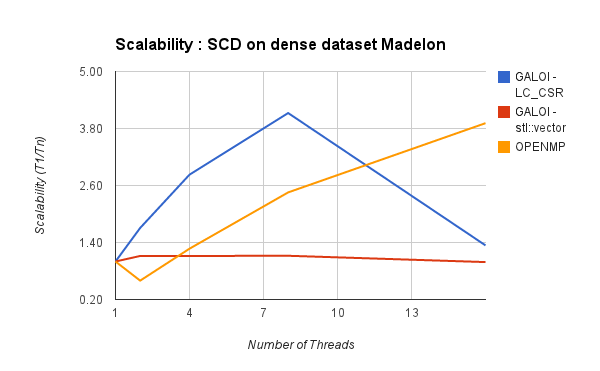
\includegraphics[width=80mm]{scd_scale_dense.png}
\caption{Scalability for Coordinate Gradient descent on dense dataset Madelon }
\label{overflow}
\end{figure}

\begin{figure}[ht!]
\centering
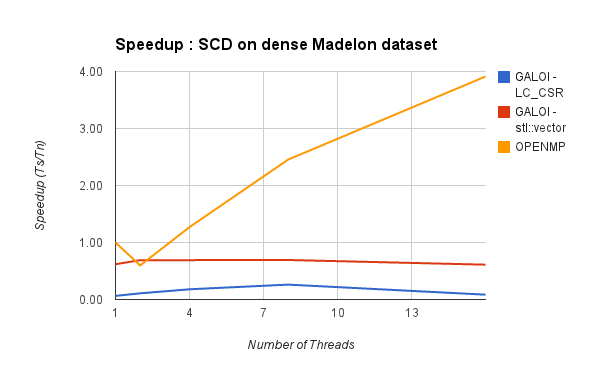
\includegraphics[width=80mm]{scd_speed_dense.png}
\caption{Speedup for Stochastic Coordinate Gradient descent on dense dataset Madelon }
\label{overflow}
\end{figure}

\begin{figure}[ht!]
\centering
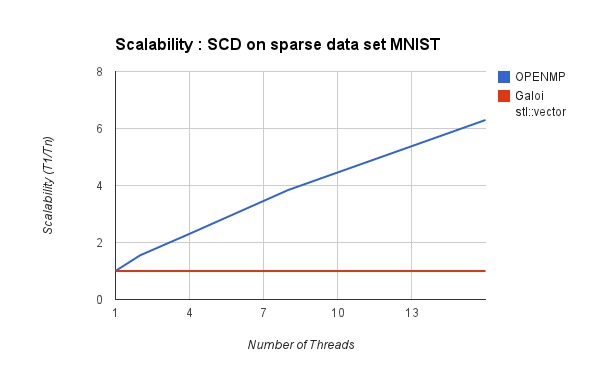
\includegraphics[width=80mm]{scd_scale_sparse.png}
\caption{Scalability for Stochastic Coordinate Gradient descent on sparse dataset MNIST }
\label{overflow}
\end{figure}

\begin{figure}[ht!]
\centering
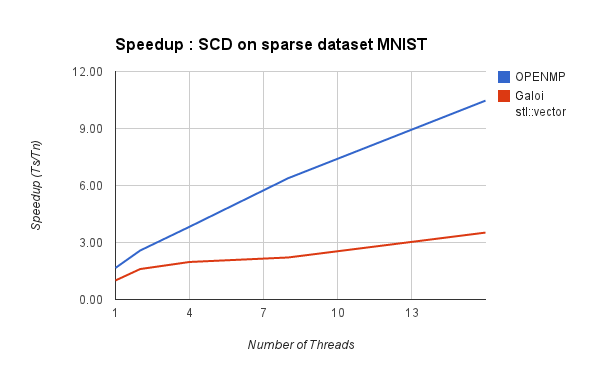
\includegraphics[width=80mm]{scd_speed_sparse.png}
\caption{Speedup for Stochastic Coordinate Gradient descent on sparse dataset MNIST }
\label{overflow}
\end{figure}

\begin{figure}[ht!]
\centering
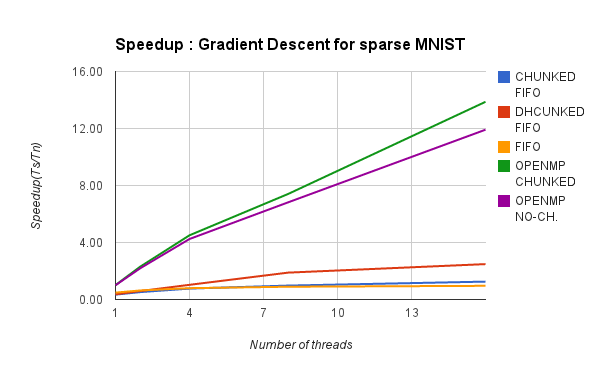
\includegraphics[width=80mm]{gd_speed_sparse.png}
\caption{Speedup for Gradient descent on sparse dataset MNIST. }
\label{overflow}
\end{figure}


\begin{figure}[ht!]
\centering
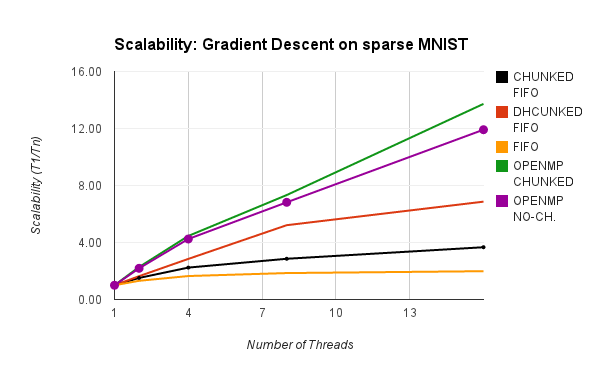
\includegraphics[width=80mm]{gd_scale_sparse.png}
\caption{Scalability for Gradient descent on sparse dataset MNIST. }
\label{overflow}
\end{figure}



\subsection{Parallel Gradient Descent}	
\begin{table}[htbp]
\caption{Run time for GD on MNIST dataset}
\begin{tabular}{|p{9em}|p{2em}|p{2em}|p{2em}|p{2em}|p{2em}|}
\hline
 & 1 & 2 & 4 & 8 & 16 \\ \hline
Galois Chunked FIFO & 45.96 & 30.36 & 20.53 & 16.08 & 12.53 \\ \hline
Galois dChunked FIFO & 43.46 & 26.55 & 15.26 & 8.33 & 6.33 \\ \hline
Galois FIFO & 32.54 & 24.79 & 19.76 & 17.54 & 16.38 \\ \hline
OPENMP & 15.72 & 7.184 & 3.70 & 2.30 & 1.31 \\ \hline
OPENMP Chunked. & 15.55 & 6.83 & 3.49 & 2.12 & 1.13 \\ \hline
\end{tabular}
\end{table}
	
	\subsubsection{Different Galois Schedules vs OpenMP}
	Table 1 shows the runtime for the Gradient Descent for sparse dataset Mnist. The minimum runtime is 
	achieved for OpenMP Chunked implementation. Figure 1 compares the Scalability for different Galois Schedules and OpenMP.
	The chunked implementations scales better compared to un-chunked version for both Galois and OpenMP. This is expected as the chunked
    	implementation distributes the samples among different threads and has less contention. For the same reason,
    	the Chunked and DChunked-FIFO Scheduling have better scalability than the FIFO scheduling. Also, OpenMP

\begin{figure}[ht!]
\centering
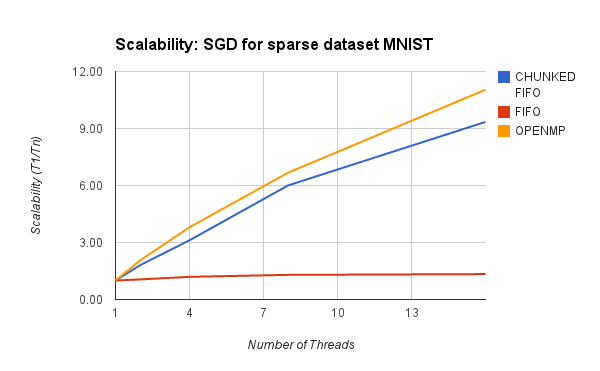
\includegraphics[width=80mm]{sgd_scale_sparse.png}
\caption{Scalability for Stochastic Gradient descent on sparse dataset MNIST. }
\label{overflow}
\end{figure}


\begin{figure}[ht!]
\centering
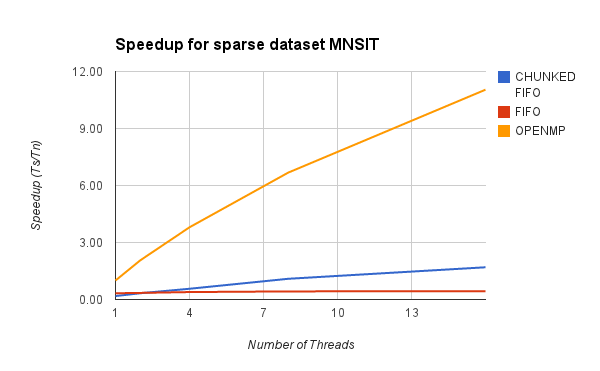
\includegraphics[width=80mm]{sgd_speed_sparse.png}
\caption{Speedup for Stochastic Gradient descent on sparse dataset MNIST. }
\label{overflow}
\end{figure}
	Table X shows the runtime for the Gradient Descent for sparse dataset Mnist. The minimum runtime is 
	achieved for OpenMP Chunked implementation. Figure X compares the Scalability for different Galois Schedules and OpenMP.
	The chunked implementations scales better compared to un-chunked version for both Galois and OpenMP. This is expected as the chunked
    	implementation distributes the samples among different threads and has less contention. For the same reason,
    	the Chunked and DChunked-FIFO Scheduling have better scalability than the FIFO scheduling. Also, OpenMP
    	scales better than Galois for both chunked and unchunked version.
     
    	\subsubsection{Different Regression Models vs Accuracy}

	Figure X compares the Error Loss for different Regression Models. The Error Loss is minimum for Least Squares
	as it tries to (mis)fit the training data the best, leading to Overfitting. The Ridge, Lasso and Elastic Net
	models penalize the objective function and thus, the Error Loss is greater than Least Squares. 
    
   	\subsubsection{No of Iterations vs Accuracy}
    	
\begin{figure}[ht!]
\centering
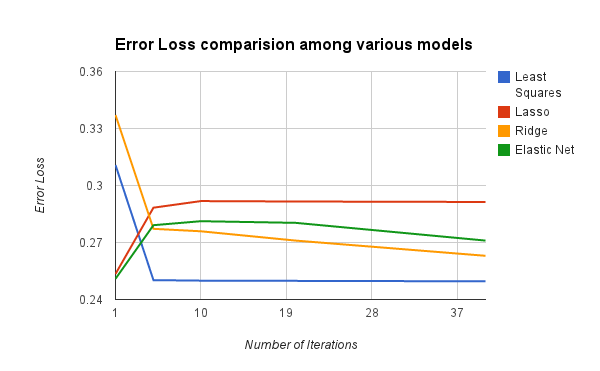
\includegraphics[width=80mm]{error_loss1.png}
\caption{ Error Loss between different Regression models. }
\label{overflow}
\end{figure}
	As can be seen from Figure X, the Error Loss function for Least Squares decreases with iterations as the models
	tries to perfectly fit the training data. The Error Loss function for Lasso and Elastic Net increases with iterations
	due to regularization.

\subsection{Parallel Stochastic Gradient Descent}
\begin{table}[htbp]
\caption{Run time for SGD on MNIST dataset}
\begin{tabular}{|p{9em}|p{2em}|p{2em}|p{2em}|p{2em}|p{2em}|}
\hline
 & 1 & 2 & 4 & 8 & 16 \\ \hline
Galois CHUNKED FIFO & 38.43 & 21.24 & 12.32 & 6.39 & 4.11 \\ \hline
Galois FIFO & 21.24 & 20.09 & 17.81 & 16.38 & 15.88 \\ \hline
OPENMP & 6.97 & 3.38 & 1.83 & 1.04 & 0.63 \\ \hline
\end{tabular}
\label{Label of the table}
\end{table}

	\subsubsection{Different Galois Schedules vs OpenMP}
	Table X and Figure X compare the runtime and scalibilty for different Galois schedules and OpenMP for Parallel SGD
	implementation. As the case with Gradient Descent, best runtime and speedup is achieved for OpenMp chunked implementation.
	Also, Chunked FIFO Galois scheduling gives much better speeup compared to FIFO scheduling for the worklist.
	
	\subsubsection{Accuracy Comparison for SGD vs GD}
	For the same number of iterations, GD is more accurate than SGD as can be seen in Figure X. This is because in one iteration
	of GD, all the samples are taken into consideration and the weight vector is updated with the mean of values computed using all
	samples. On the contrary, in SGD only one sample is considered in each iteration. This also means that SGD is a lot faster compared
	to GD for the same number of iterations. Also, SGD converges faster than GD due to immediate update of values but runs a higher
	risk of divergence.

	\subsubsection{Error Rate Variation with Learning Rate \(\eta\) }
	The key insight in Figure X is that the Error loss function oscillates more for a bigger value of the Learning Rate (neta).
	As can be seen, Error loss oscillates the most for a neta value of 0.01. For neta equals to 0.001, the Error loss converges faster
	as compared to 0.0001 but it oscillates more as well.

\subsection{Parallel Stochastic Coordinate Descent}
\begin{table}[htbp]
\caption{Runtime for SCD on Madelon dataset}
\begin{tabular}{|p{7em}|p{2.5em}|p{2.5em}|p{2.5em}|p{2em}|p{2.5em}|}
\hline
 & 1 & 2 & 4 & 8 & 16 \\ \hline
Galois - LC\_CSR & 349.69 & 204.94 & 123.65 & 84.76 & 261.08 \\ \hline
Galois - STL::Vector  & 35.80 & 32.06 & 32.06 & 31.95 & 36.24 \\ \hline
OPENMP & 22.14 & 37.08 & 17.44 & 9.02 & 5.66 \\ \hline
\end{tabular}
\label{Label of the table}
\end{table}

\begin{table}[htbp]
\caption{Runtime for SCD on MNIST dataset}
\begin{tabular}{|p{7em}|p{2.5em}|p{2.5em}|p{2.5em}|p{2em}|p{2.5em}|}
\hline
 & 1 & 2 & 4 & 8 & 16 \\ \hline
Galois STL::Vector & 206.14 & 205.62 & 206.20 & 205.67 & 205.42 \\ \hline
OPENMP & 124.04 & 79.97 & 53.85 & 32.29 & 19.69 \\ \hline
\end{tabular}
\label{Label of the table}
\end{table}


\subsubsection{Different Galois Schedules vs OpenMP}
Tables X \& X show that the OpenMP implementation has lesser runtime than Galois. This is in accordance with the results seen for the Gradient
algorithms. Also the LC\_CSR\_Graph implementation is slower than the STL::Vector implementation. 

\section{Conclusion}
Gradient Descent, Coordinate Descent and their parallel Stochastic versions were implemented on OpenMP and Galois systems. The runtimes and speedup
were compared for OpenMP and Galois and it was concluded that OpenMP had lesser runtime than Galois in all cases. Also, the chunked implementations
were faster than the non-Chunked ones for both Galois and OpenMP. Also, the Error loss function was least for Least Squares Regression implying that it
(mis)fits the training data the most. The Error loss function decreases with the number of iterations for Least Squares leading to Overfitting. The Stochastic
Gradient Descent converges faster than Gradient descent because of the online updation of weight values. Last but not the least, a larger value of learning
rate \(\eta\) leads to faster convergence rate but causes lot more oscillations and an increased risk of divergence.

% We recommend abbrvnat bibliography style.
%\bibliographystyle{unsrt}

\bibliographystyle{abbrvnat}
% The bibliography should be embedded for final submission.

\begin{thebibliography}{}
\softraggedright

\bibitem[Niu et~al.(2011)Niu, F.]{hogwild}
Niu F. and Recht B., Hogwild!: A Lock-Free Approach to Parallelizing Stochastic Gradient Descent.
\bibitem[Zhang et~al.(2004) Zhang, T.]{zhang1}
Zhang T., Solving Large Scale Linear Prediction Problems Using Stochastic Gradient Descent Algorithms.
\bibitem[Richtarik et~al.(2012) Richtarik, P.]{rich1}
Richtarik P., and Takac M., Parallel Coordinate Descent methods for Big Data Optimization.
\bibitem[Friedman et~al.(2007) Friedman, J.]{pcd1}
J. Friedman, T. Hastie, H. Hoeing, and R. Tibshirani, Pathwise coordinate optimization.
\bibitem[Fu et~al.(1998) Fu, W.]{fu1}
T. Wu and K. Lange, Coordinate descent algorithms for lasso penalized regression.
\bibitem[Tewari et~al.(2008) Wu, T.]{tewari}
Stochastic methods for l1 regularized loss minimization
\bibitem[Tewari et~al.(2008) Wu, T.]{shotgun}
Parallelized Coordinate Descent for L-1 regularized loss minimization!
\bibitem[Pingali et~al. ] {galois1}
Keshav Pingali , Donald Nguyen , Milind Kulkarni , Martin Burtscher , M. Amber Hassaan , Rashid
Kaleem , Tsung-Hsien Lee , Andrew Lenharth , Roman Manevich , Mario Méndez-Lojo , Dimitrios
Prountzos , Xin Sui, The tao of parallelism in algorithms, Proceedings of the 32nd ACM SIGPLAN
conference on Programming language design and implementation, June 04-08, 2011, San Jose,
California, USA
\bibitem[Blas library ] {blas}
Basic Linear Algebra Subprograms for Fortran Usage.
\bibitem[OpenMP ] {openmp}
http://openmp.org/wp/
\bibitem[OpenMP ] {galois2}
http://iss.ices.utexas.edu/?p=projects/galois
\bibitem[sckit-learn ] {scikit}
http://scikit-learn.org/stable/

\end{thebibliography}

\acks
Thanks to our machine learning expert Si Si for guiding us through the process of learning about different regression algorithms, Xin Sui for giving us useful information on Galois and Prof. Pingali for giving us the initial push.


\end{document}

%                       Revision History
%                       -------- -------
%  Date         Person  Ver.    Change
%  ----         ------  ----    ------

%  2013.06.29   TU      0.1--4  comments on permission/copyright notices

